\chapter{分段母线(非环网)继电保护逻辑图分析}
现有一分段母线(非环网)的继电保护逻辑图如:

% TODO: \usepackage{graphicx} required
\begin{figure}[h]
	\centering
	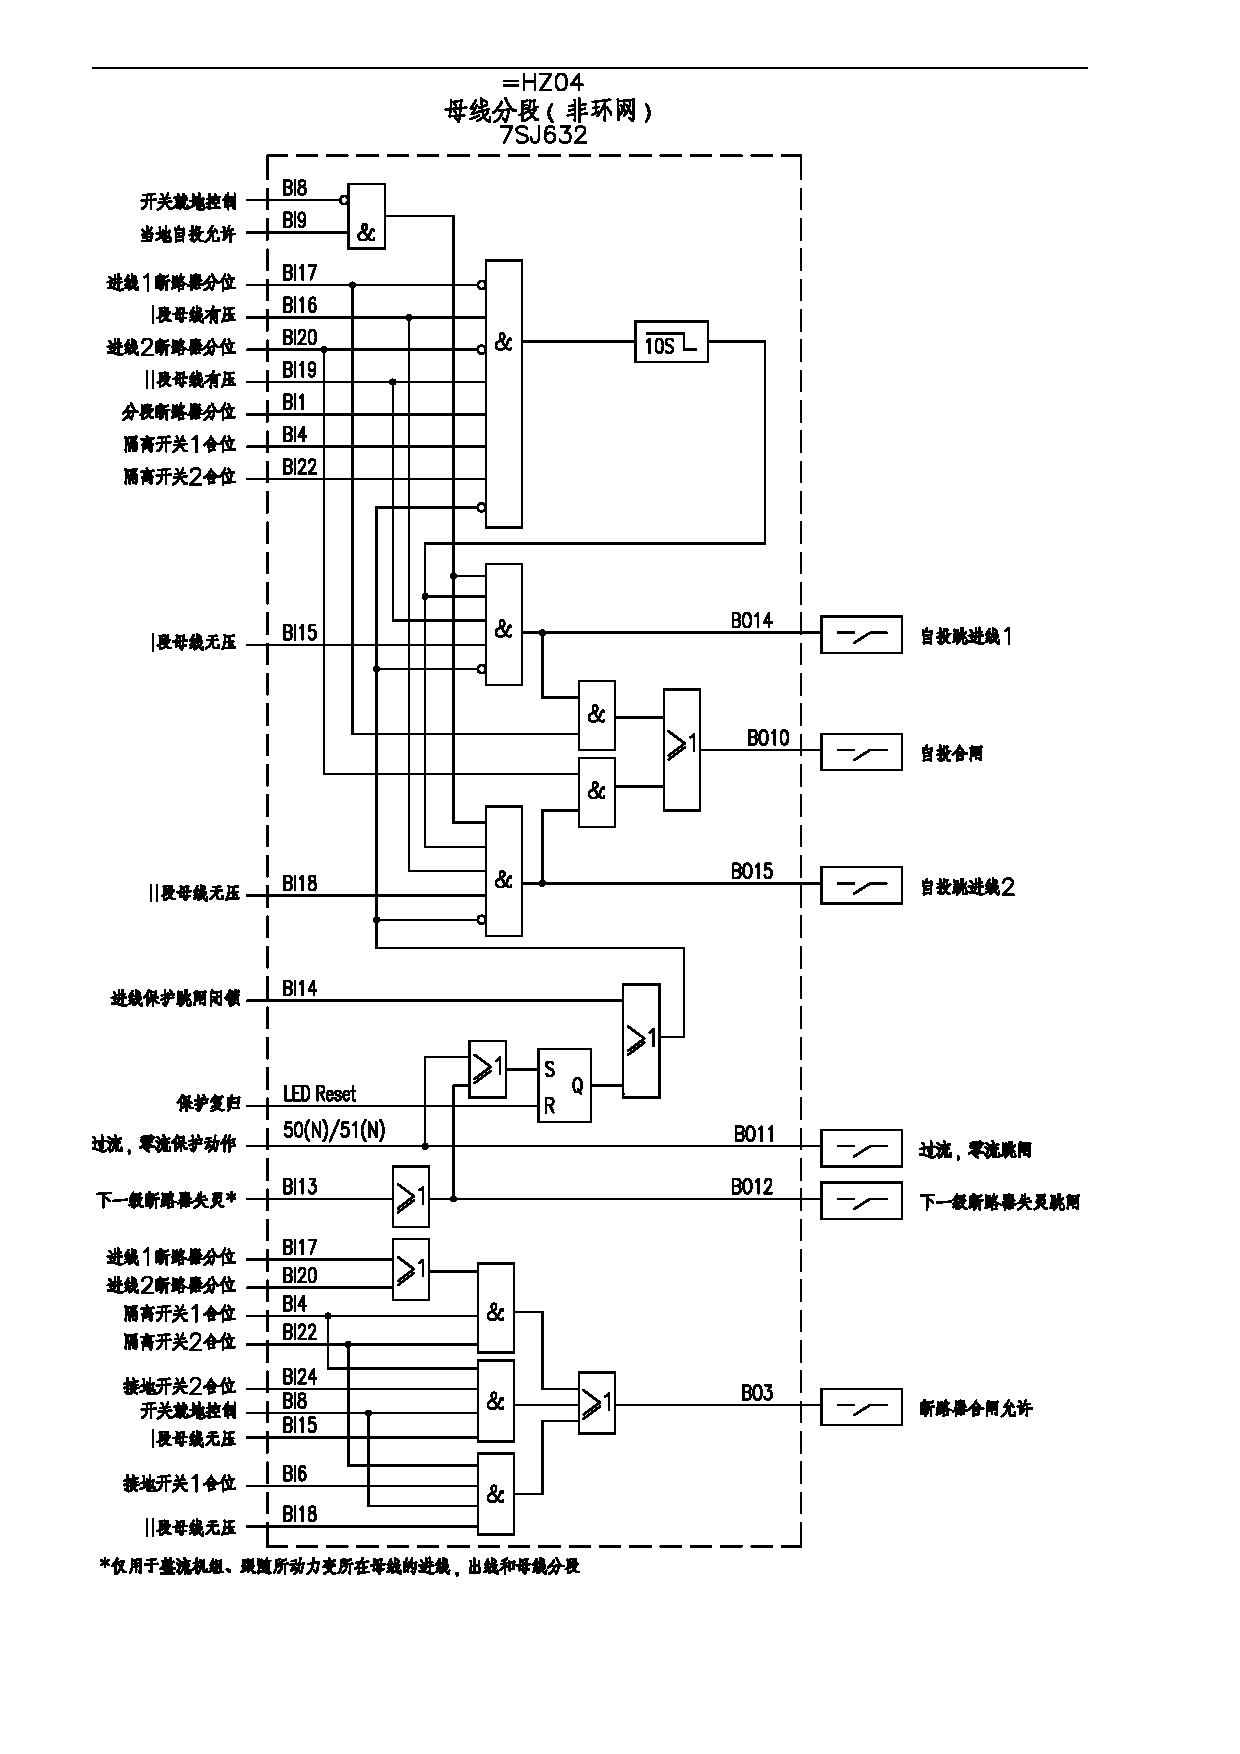
\includegraphics[width=0.7\linewidth]{figures/分段母线(非环网)的继电保护逻辑图}
	\caption{分段母线(非环网)的继电保护逻辑图}
	\label{fig:分段母线(非环网)的继电保护逻辑图}
\end{figure}

由于该图左侧输入相比于右侧输出复杂得多,于是从右侧向左侧反推,找出各种输出所对应的条件即可完成分析。

\section{10s维持触发}
10s维持触发需要满足的条件如下:

\begin{enumerate}
	\item 进线1断路器处于合位。
	\item I段母线有压。
	\item 进线2断路器处于合位。
	\item I段母线有压。
	\item 分段断路器处于分位。
	\item 隔离开关1处于合位。
	\item 隔离开关2处于合位。
	\item 进线保护跳闸闭锁且保护复归,过流、零序保护不动作,下一级断路器正常。
\end{enumerate}

\section{自投跳进线1}
若自投跳进线1动作,则:

\begin{enumerate}
	\item I段母线失压。
	\item II段母线正常有压。
	\item 10秒维持触发处于触发状态。
	\item 开关就地控制打至0位且当地自投允许打自1位。
	\item 进线保护跳闸闭锁且保护复归,过流、零序保护不动作,下一级断路器正常。
\end{enumerate}

\section{自投合闸}
若自投合闸动作,则有下列两者情况之一或同时发生:

\begin{enumerate}
	\item 自投跳进线1动作且进线1断路器处于分位。
	\item 进线2断路器处于分位且自投跳进线2动作。
\end{enumerate}

\section{自投跳进线2}
若自投跳进线2动作,则:

\begin{enumerate}
	\item II段母线无压。
	\item I段母线有压。
	\item 10秒维持触发处于触发状态。
	\item 开关就地控制打至0位且当地自投允许打自1位。
	\item 进线保护跳闸闭锁且保护复归,过流、零序保护不动作,下一级断路器正常。
\end{enumerate}

\section{过滤零流跳闸}
若过滤零流跳闸动作,则有:

\begin{enumerate}
	\item 过流零流保护动作。
\end{enumerate}

\section{下一级断路器失灵跳闸}

若下一级断路器失灵B113输出动作信号,B102通过动作信号。

\section{断路器合闸允许}
断路器合闸允许需要满足以下条件之一:

\begin{enumerate}
	\item 进线1断路器或进线2断路器处于分位且隔离开关1和隔离开关2均处于合位。
	\item 隔离开关1处于合闸位且有接地开关2处于合位,开关就地控制打至1位,I段母线无压。
	\item 隔离开关2处于合闸位且有接地开关1处于合位,开关就地控制打至1位,II段母线无压。
\end{enumerate}
